\documentclass[10pt,a4paper,twocolumn]{article}

% ─── Packages ──────────────────────────────────────────────────────────────
\usepackage[a4paper, top=1.8cm, bottom=1.8cm, left=1.5cm, right=1.5cm,
            columnsep=0.6cm]{geometry}
\usepackage{amsmath, amssymb, amsthm}
\usepackage{graphicx}
\usepackage{booktabs}
\usepackage{multirow}
\usepackage{array}
\usepackage{tabularx}
\usepackage{xcolor}
\usepackage[hidelinks]{hyperref}
\usepackage{natbib}
\usepackage{microtype}
\usepackage{enumitem}
\usepackage{caption}
\usepackage{subcaption}
\usepackage{float}
\usepackage{algorithm}
\usepackage{algpseudocode}
\usepackage{tikz}
\usepackage{pgfplots}
\pgfplotsset{compat=1.18}
\usepackage{mdframed}
\usepackage{setspace}
\usepackage{fancyhdr}
\usepackage{titlesec}
\usepackage{parskip}
\usepackage{balance}

% ─── Color definitions ──────────────────────────────────────────────────────
\definecolor{accentblue}{RGB}{20, 70, 150}
\definecolor{boxgray}{RGB}{245, 245, 248}
\definecolor{methgreen}{RGB}{0, 110, 70}

% ─── Section formatting ─────────────────────────────────────────────────────
\titleformat{\section}{\normalsize\bfseries\color{accentblue}}{\thesection}{0.5em}{}[\vspace{-2pt}\titlerule\vspace{2pt}]
\titleformat{\subsection}{\small\bfseries}{\thesubsection}{0.5em}{}
\titleformat{\subsubsection}[runin]{\small\bfseries\itshape}{\thesubsubsection}{0.4em}{}[.\enspace]
\titlespacing{\section}{0pt}{6pt}{3pt}
\titlespacing{\subsection}{0pt}{4pt}{2pt}

% ─── Header / footer ────────────────────────────────────────────────────────
\pagestyle{fancy}\fancyhf{}
\lhead{\scriptsize Interpretable Disease--Gene Prediction via Hybrid Graph Learning}
\rhead{\scriptsize CentraleSupelec, 2025}
\rfoot{\scriptsize\thepage}
\renewcommand{\headrulewidth}{0.3pt}
\setlength{\headheight}{12pt}

% ─── Paragraph / float spacing ──────────────────────────────────────────────
\setlength{\parskip}{3pt}
\setlength{\parindent}{0pt}
\setlength{\abovecaptionskip}{4pt}
\setlength{\belowcaptionskip}{2pt}
\setlength{\floatsep}{6pt}
\setlength{\textfloatsep}{6pt}
\captionsetup{font=scriptsize, labelfont=bf}

% ─── Def box ────────────────────────────────────────────────────────────────
\newmdenv[backgroundcolor=boxgray, linewidth=0.6pt, linecolor=accentblue!40,
          innerleftmargin=6pt, innerrightmargin=6pt,
          innertopmargin=4pt, innerbottommargin=4pt,
          skipabove=4pt, skipbelow=4pt]{defbox}

% ─── Math operators ─────────────────────────────────────────────────────────
\DeclareMathOperator{\CN}{CN}
\DeclareMathOperator{\AAd}{AA}
\newcommand{\Gcal}{\mathcal{G}}
\newcommand{\Vcal}{\mathcal{V}}
\newcommand{\Ecal}{\mathcal{E}}
\newcommand{\Rcal}{\mathcal{R}}

% ─── Title ──────────────────────────────────────────────────────────────────
\title{\vspace{-1.2cm}{\large\bfseries Interpretable Disease--Gene Prediction via\\
Hybrid Graph Learning and Metapath Reasoning}\\[4pt]
{\small Project Final Report --- Graph Learning, CentraleSupelec 2025}}
\author{\small Farouk Yartaoui \quad Hala Chafik \quad Hamza Tbatou \quad Ilyas Maddah}
\date{}

% ============================================================================
\begin{document}
\maketitle\thispagestyle{fancy}
\vspace{-10pt}

% ─── Abstract ───────────────────────────────────────────────────────────────
\begin{mdframed}[backgroundcolor=boxgray, linewidth=0pt,
  innerleftmargin=6pt, innerrightmargin=6pt,
  innertopmargin=5pt, innerbottommargin=5pt]
\small\textbf{Abstract.}
Predicting associations between diseases and genes is a foundational challenge
in biomedical research, with direct applications in drug discovery, variant
prioritisation, and personalised medicine. Most existing approaches either
achieve strong predictive performance at the expense of interpretability (e.g.\
deep graph neural networks), or provide transparent reasoning through
hand-crafted features without the capacity to learn (e.g.\ metapath-based
logistic regression). We bridge this gap on the Hetionet v1.0 heterogeneous
biomedical knowledge graph by evaluating a suite of methods --- structural graph
heuristics (Common Neighbours, Adamic--Adar), shallow random-walk embeddings
(Node2Vec), and a Heterogeneous Attention Network (HAN) --- and by proposing a
lightweight \emph{hybrid model} that linearly interpolates GNN link-prediction
scores with biologically motivated metapath path-count evidence. The
interpolation scalar $\alpha$ is optimised on a held-out validation set, adding
no trainable parameters beyond those of the GNN. We evaluate on AUC-ROC,
AUC-PR, Hits@$k$, and MRR over three random seeds, and complement quantitative
results with an interpretability analysis cross-referencing top predictions
against OMIM and KEGG. The hybrid model outperforms all individual baselines,
and 70\% of top-20 predictions are externally supported by biological databases,
confirming the method's capacity to generate actionable, interpretable
hypotheses.
\end{mdframed}

% ============================================================================
\section{Introduction and Motivation}
\label{sec:intro}
% ============================================================================

Understanding which genes are implicated in which diseases is central to modern
biomedicine. The human genome encodes roughly 20{,}000 protein-coding genes, yet
experimentally confirmed gene--disease associations remain sparse and
concentrated around a small set of well-studied conditions. Bridging this gap
has far-reaching consequences.

\textbf{Applications.} Accurate disease--gene prediction directly supports:
(i)~\textit{drug target identification}, by nominating causal genes for
therapeutic intervention; (ii)~\textit{genomic variant prioritisation} in
clinical sequencing pipelines, by ranking candidate variants by disease
relevance; (iii)~\textit{drug repurposing}, by identifying off-target disease
associations of existing compounds; and (iv)~\textit{personalised medicine}, by
tailoring treatment to individual genetic profiles.

\textbf{Core challenge.} State-of-the-art graph neural networks excel at
capturing latent structural patterns but produce predictions that are difficult
to explain --- a critical shortcoming in biomedical settings where a wet-lab
scientist must decide which candidates to pursue experimentally. Conversely,
interpretable methods based on explicit relational paths sacrifice predictive
power. This tension motivates our hybrid approach.

\textbf{Research questions.} We address three questions: (1)~How do graph
heuristics, shallow embeddings, and heterogeneous GNNs compare on disease--gene
link prediction? (2)~Can explicit metapath path-count evidence complement GNN
predictions to improve ranking performance? (3)~What fraction of top predictions
can be biologically validated, and which relational patterns are most
explanatory?

% ============================================================================
\section{Problem Definition}
\label{sec:problem}
% ============================================================================

\textbf{Notation.} Let $\Gcal = (\Vcal, \Ecal, \phi, \psi)$ be a
\textit{heterogeneous graph} where $\phi : \Vcal \to \mathcal{A}$ maps nodes to
types and $\psi : \Ecal \to \Rcal$ maps edges to relation types, with
$|\mathcal{A}| > 1$ or $|\Rcal| > 1$. Let $\Vcal_D \subset \Vcal$ and
$\Vcal_G \subset \Vcal$ denote disease and gene node sets respectively. We
denote the known positive association set as $\Ecal^+ \subset \Vcal_D \times
\Vcal_G$.

\begin{defbox}
\textbf{Task (Disease--Gene Link Prediction).}
Given $\Gcal$ with a subset of $\Ecal^+$ hidden as the test set, learn a scoring
function $f : \Vcal_D \times \Vcal_G \to \mathbb{R}$ such that $f(d,g) > f(d,g')$
whenever $(d,g) \in \Ecal^+$ and $(d,g') \notin \Ecal^+$. We optimise for
AUC-PR on a held-out validation set.
\end{defbox}

\textbf{Constraints and assumptions.} The task is \textit{transductive}: the
full graph $\Gcal$ minus hidden edges is available at training time. We adopt the
standard open-world assumption --- unobserved pairs are treated as unknown
rather than confirmed negatives~\citep{nickel2016review}. No node features
beyond structural identity are assumed, so all signal must come from graph
topology and relational structure.

\textbf{Hardness.} Link prediction on heterogeneous graphs is NP-hard in the
general case of exact optimal ranking~\citep{liben2007link}. Practical
difficulty arises from: (i)~severe class imbalance ($|\Ecal^+| \approx 12{,}000$
against a candidate space of $|\Vcal_D| \times |\Vcal_G| \approx 1.8 \times
10^6$); (ii)~heterogeneity requiring type-aware models; and (iii)~the
open-world assumption making it impossible to distinguish true from unknown
negatives.

\textbf{Optimisation objective.} We train models to minimise binary
cross-entropy over labelled edge pairs:
\begin{equation}
\mathcal{L} = -\!\!\sum_{(d,g,y)}\!\left[y\log f(d,g)+(1-y)\log(1-f(d,g))\right]
\label{eq:loss}
\end{equation}
The scalar $\alpha$ in the hybrid model is separately optimised by grid search
on validation AUC-PR.

% ============================================================================
\section{Related Work}
\label{sec:related}
% ============================================================================

\textbf{Himmelstein et al.\ (2017)~\citep{himmelstein2017}} construct Hetionet
by integrating 29 biomedical databases and propose \textit{Degree-Weighted Path
Counts} (DWPC) along metapaths as features for logistic regression. This is our
closest methodological ancestor: we adopt its dataset and metapath philosophy,
but replace logistic regression with a learned GNN and fuse the two. Relevant
as the source of our dataset, the DWPC scoring baseline, and the interpretability
framework we extend.

\textbf{Kipf \& Welling (2017)~\citep{kipf2017gcn}} introduce Graph
Convolutional Networks (GCN), learning node representations by propagating
features through spectral graph convolution. Relevant as the foundational GNN
architecture whose message-passing paradigm underlies all subsequent methods
including HAN and R-GCN.

\textbf{Wang et al.\ (2019)~\citep{wang2019han}} propose the Heterogeneous
Attention Network (HAN), which aggregates node neighbourhoods along metapaths
via a two-level attention mechanism (node-level and semantic-level). It is our
primary GNN baseline, purpose-built for multi-type graphs and capable of
softly weighting metapath contributions. As noted by~\citet{adnan2024benchmark},
HAN does not always outperform simpler methods on biomedical tasks, motivating
the hybrid extension.

\textbf{Grover \& Leskovec (2016)~\citep{grover2016node2vec}} introduce
Node2Vec, learning embeddings via biased second-order random walks and a
skip-gram objective. Relevant as the standard scalable shallow-embedding
baseline: its performance gap relative to HAN isolates the value of type-aware
relational modelling.

\textbf{Himmelstein et al.\ (2022)~\citep{himmelstein2022}} propose the Hetnet
Connectivity Search, an unsupervised system that retrieves enriched connecting
paths between Hetionet nodes without supervised training. It demonstrates that
path evidence alone recovers much of the supervised model's performance, directly
motivating our decision to add explicit metapath counts to the GNN score.
Relevant as evidence that interpretable path-based signals are powerful and
complementary to learned representations.

\textbf{Schlichtkrull et al.\ (2018)~\citep{schlichtkrull2018rgcn}} propose
R-GCN, handling multi-relational graphs via relation-specific weight matrices.
Relevant as an alternative heterogeneous GNN; we use HAN over R-GCN for its
explicit metapath semantics and attention-based interpretability.

\textbf{Gap.} No prior work jointly combines a trained GNN with explicit
metapath path-count evidence in a unified, parameter-efficient scoring pipeline
targeting both accuracy and interpretability for disease--gene prioritisation on
Hetionet. Our hybrid model fills this gap.

% ============================================================================
\section{Methodology}
\label{sec:methodology}
% ============================================================================

\subsection{Data and Preprocessing}

\textbf{Hetionet v1.0}~\citep{himmelstein2017} integrates 29 public databases
into a large-scale heterogeneous biomedical graph. We restrict to the four node
types most relevant to disease--gene association (Table~\ref{tab:data}) and
exclude compound nodes, which expand the graph substantially without
participating in our disease--gene metapaths.

\begin{table}[H]
\centering\scriptsize
\caption{Hetionet subgraph statistics.}
\label{tab:data}
\setlength{\tabcolsep}{3pt}
\begin{tabular}{lrp{2.4cm}}
\toprule
\textbf{Node type} & \textbf{Count} & \textbf{Key edge types (count)} \\
\midrule
Gene      & ${\approx}13{,}000$ & assoc.\ Disease (${\approx}12$k) \\
Disease   & ${\approx}137$      & presents Phenotype (${\approx}4.6$k) \\
Pathway   & ${\approx}1{,}400$  & Gene participates (${\approx}85$k) \\
Phenotype & ${\approx}9{,}000$  & Gene covaries Gene (${\approx}61$k) \\
\bottomrule
\end{tabular}
\end{table}

\textbf{Graph construction.} Two parallel representations are built: (a)~a
\texttt{NetworkX MultiDiGraph} retaining all edge types, used for BFS-based
metapath counting; (b)~a PyTorch Geometric \texttt{HeteroData} object with
one-hot type vectors as node features and per-type edge index tensors, used for
GNN training. A homogeneous projection (edge types ignored) is built for
Node2Vec.

\textbf{Edge splitting.} Positive \textit{Gene--associates--Disease} edges are
split 80/10/10 (train/val/test), stratified so every test disease has at least
one training positive. Negatives are sampled at a 1:5 ratio: for each disease in
a split, 5 genes not known to associate with that disease are drawn uniformly.
All experiments repeat over $S=3$ random seeds.

\textbf{Metapath caching.} BFS path counting is pre-computed and cached to disk
via \texttt{joblib.Memory}, reducing repeated runtime from ${\sim}4$ hours to
${\sim}25$ minutes on 16 cores.

\subsection{Graph Heuristics}

Heuristics provide parameter-free, fast baselines. We project the heterogeneous
graph to a bipartite disease--gene neighbourhood via shared intermediate nodes
(pathways, phenotypes, co-varying genes) to define common neighbours $N(\cdot)$.

\textit{Common Neighbours (CN)} counts shared biological intermediates:
\begin{equation}
s_{\CN}(d,g) = |N(d) \cap N(g)|
\label{eq:cn}
\end{equation}
The intuition is that a disease and gene sharing many intermediate entities
(e.g.\ pathways, phenotypes) are likely functionally related. CN is competitive
on sparse graphs with few hubs.

\textit{Adamic--Adar (AA)}~\citep{adamic2003aa} downweights high-degree shared
neighbours:
\begin{equation}
s_{\AAd}(d,g) = \sum_{u \in N(d) \cap N(g)} \frac{1}{\log |N(u)|}
\label{eq:aa}
\end{equation}
Sharing a rare pathway (small $|N(u)|$) is more informative than sharing a
ubiquitous hub, directly mirroring the DWPC philosophy~\citep{himmelstein2017}.

\textbf{Merging.} Both scores are min-max normalised per disease and linearly
combined: $s_{\text{heur}} = \beta\hat{s}_{\CN} + (1-\beta)\hat{s}_{\AAd}$,
with $\beta$ selected by validation AUC-PR ($\beta\approx0.5$ empirically).

\textbf{Intuition and limitations.} Heuristics are fully interpretable and
parameter-free, making them excellent sanity checks. However, they cannot learn
non-linear interactions between relational patterns and are blind to information
more than 2 hops away from the query pair.

\subsection{Node2Vec}

Node2Vec~\citep{grover2016node2vec} learns $d$-dimensional node embeddings by
optimising a skip-gram objective over biased second-order random walks. Given
current node $v$ and previous node $t$, the unnormalised probability of
transitioning to neighbour $x$ is:
\begin{equation}
\pi_{vx} = \alpha_{pq}(t,x)\cdot w_{vx},\;\;
\alpha_{pq}(t,x) = \begin{cases}
1/p & d_{tx}=0 \\ 1 & d_{tx}=1 \\ 1/q & d_{tx}=2
\end{cases}
\end{equation}
where $d_{tx}$ is the shortest-path distance from $t$ to $x$. Parameter $p$
controls the return probability; $q$ balances local (BFS-like, $q<1$) vs.\
global (DFS-like, $q>1$) exploration. The skip-gram objective maximises:
\begin{equation}
\max_\mathbf{f} \sum_{v\in\Vcal}\sum_{u\in N_S(v)} \mathbf{f}(u)^\top\mathbf{f}(v) - \log Z(v)
\end{equation}
with $Z(v)$ approximated by negative sampling. Link scores:
$s_{\text{N2V}}(d,g) = \sigma(\mathbf{f}(d)^\top\mathbf{f}(g))$.

\textbf{Why Node2Vec?} It captures global graph topology without a complex
training pipeline or metapath specification, serving as an upper bound on how
much information is available in bare graph structure, independent of edge types.
This makes its performance directly comparable to type-aware methods as an
ablation of the value of edge-type information.

\subsection{Heterogeneous Attention Network (HAN)}

HAN~\citep{wang2019han} is purpose-built for heterogeneous graphs. It projects
the graph into metapath-induced homogeneous subgraphs, applies graph attention
within each, then fuses representations across metapaths via learned semantic
attention.

\textbf{Metapath-induced graphs.} Given a metapath $\Phi$, the induced graph
$\Gcal_\Phi$ connects two nodes of the same type if a path of type $\Phi$
exists between them. We use three HAN metapaths: \texttt{GaDaG} (genes
co-associated via a disease), \texttt{DaGaD} (diseases co-associated via a
gene), and \texttt{GpPpG} (genes sharing a pathway).

\textbf{Node-level attention.} For node $v$ and metapath $\Phi$, the attention
weight of neighbour $u \in \mathcal{N}_v^\Phi$ is:
\begin{equation}
\alpha_{vu}^\Phi = \frac{
  \exp\!\bigl(\text{LeakyReLU}(\mathbf{a}_\Phi^\top[\mathbf{W}_\Phi\mathbf{h}_v \| \mathbf{W}_\Phi\mathbf{h}_u])\bigr)
}{
  \sum_{k\in\mathcal{N}_v^\Phi}\exp(\cdots)
}
\end{equation}
giving metapath embedding $\mathbf{z}_v^\Phi = \sigma\!\bigl(\sum_u \alpha_{vu}^\Phi \mathbf{W}_\Phi\mathbf{h}_u\bigr)$.

\textbf{Semantic-level attention.} Metapath importance:
\begin{equation}
\beta_{\Phi_i} = \frac{
  \exp\!\bigl(\tfrac{1}{|\Vcal|}\sum_v \mathbf{q}^\top\tanh(\mathbf{W}\mathbf{z}_v^{\Phi_i}+\mathbf{b})\bigr)
}{
  \sum_j\exp(\cdots)
}
\end{equation}
Final embedding: $\mathbf{Z}_v = \sum_i \beta_{\Phi_i}\mathbf{z}_v^{\Phi_i}$.
Link scores: $s_{\text{HAN}}(d,g) = \sigma(\mathbf{Z}_d^\top\mathbf{Z}_g)$.

\textbf{Training details.} 2-layer HAN, hidden dim 64, 4 attention heads,
dropout 0.3, Adam ($\text{lr}=10^{-3}$, weight decay $10^{-4}$), up to 100
epochs with early stopping on validation AUC-PR (patience 10).

\subsection{Metapath Scoring}

\textbf{What are metapaths?} A metapath is a typed path in the schema graph
that encodes a specific biological hypothesis about how a disease and gene
might be related. Choosing metapaths requires domain knowledge: each metapath
must correspond to a plausible mechanistic pathway.

\textbf{Metapath selection.} We define three metapaths (Table~\ref{tab:mp}),
chosen based on biological literature and the available edge types in Hetionet.

\begin{table}[H]
\centering\scriptsize
\caption{Metapath definitions and biological rationale. $D$=Disease, $G$=Gene,
$P$=Pathway, $H$=Phenotype.}
\label{tab:mp}
\setlength{\tabcolsep}{3pt}
\begin{tabular}{p{1.3cm}lp{3.2cm}}
\toprule
\textbf{Name} & \textbf{Schema} & \textbf{Biological rationale} \\
\midrule
\texttt{DaGpPpG} &
$D\!\xrightarrow{a}\!G'\!\xrightarrow{p}\!P\!\xrightarrow{p^{-1}}\!G$ &
Candidate $G$ shares a biological pathway $P$ with a known disease gene $G'$.
Shared pathway membership is a well-established functional relatedness proxy. \\[3pt]
\texttt{DpHpG} &
$D\!\xrightarrow{\text{pr}}\!H\!\xleftarrow{\text{pr}}\!G$ &
Candidate $G$ is linked to phenotypes $H$ that disease $D$ presents.
Phenotype-gene links indicate tissue or function relevance. \\[3pt]
\texttt{GcGaD} &
$G\!\xrightarrow{c}\!G'\!\xrightarrow{a^{-1}}\!D$ &
Candidate $G$ co-varies with a known disease gene $G'$. Co-expression or
co-evolution implies shared functional roles. \\
\bottomrule
\end{tabular}
\end{table}

\textbf{Degree-downweighted path counting.} For pair $(d,g)$ and metapath
$\Phi_k$, we count instances via BFS with degree downweighting following
DWPC~\citep{himmelstein2017}:
\begin{equation}
\tilde{c}_k(d,g) = \sum_{\rho:\Phi_k,d\to g}
\prod_{e\in\rho} \frac{1}{\sqrt{\deg(\text{src}(e))\cdot\deg(\text{dst}(e))}}
\end{equation}
This penalises paths through high-degree hub nodes, which would otherwise
inflate counts uninformatively.

\textbf{Weighted scoring.} Weights $w_k$ are learned by logistic regression on
training-set path-count features, then the metapath score is:
\begin{equation}
s_{\text{path}}(d,g) = \sum_{k=1}^{3} w_k \cdot \tilde{c}_k(d,g)
\label{eq:path}
\end{equation}

\subsection{Hybrid Model}

The hybrid model fuses GNN and metapath signals via a single interpretable
scalar $\alpha \in [0,1]$:
\begin{equation}
\boxed{s_{\text{final}}(d,g) = \alpha \cdot s_{\text{GNN}}(d,g) + (1-\alpha)\cdot s_{\text{path}}(d,g)}
\label{eq:hybrid}
\end{equation}
Both scores are min-max normalised to $[0,1]$ over the validation candidate
set before combination. The scalar $\alpha$ is selected by grid search over
$\{0.0, 0.1, \ldots, 1.0\}$ maximising validation AUC-PR (Algorithm~\ref{alg:hybrid}).

\begin{algorithm}[H]
\caption{Hybrid Scoring Pipeline}
\label{alg:hybrid}
\small
\begin{algorithmic}[1]
\Require Graph $\Gcal$, train/val/test splits, trained HAN, weights $\{w_k\}$
\State Compute $\tilde{c}_k(d,g)$ for all $(d,g)$ via cached BFS
\State Get $s_{\text{GNN}}$ from trained HAN decoder on val candidates
\State Compute $s_{\text{path}}$ via Eq.~\eqref{eq:path}; normalise both to $[0,1]$
\For{$\alpha \in \{0.0, 0.1, \ldots, 1.0\}$}
  \State Evaluate AUC-PR on val using Eq.~\eqref{eq:hybrid}
\EndFor
\State $\alpha^* \leftarrow \arg\max_\alpha \text{AUC-PR}_{\text{val}}$
\State Evaluate $s_{\text{final}}$ with $\alpha^*$ on test set
\end{algorithmic}
\end{algorithm}

The design is deliberately minimal: $\alpha$ adds exactly one parameter beyond
the GNN, preserving full legibility of the metapath contribution. At $\alpha=1$
the model reduces to pure HAN; at $\alpha=0$ to pure metapath scoring.

% ============================================================================
\section{Evaluation}
\label{sec:eval}
% ============================================================================

\subsection{Metrics}

We evaluate with four complementary metrics:

\textbf{AUC-ROC} measures ranking quality across all thresholds; a global
discriminability summary robust to the class imbalance ratio used.

\textbf{AUC-PR} (primary metric) is sensitive to the 1:5 class imbalance.
A high value means top-ranked candidates are predominantly true positives ---
the operational requirement for gene prioritisation tools.

\textbf{Hits@$k$} measures the fraction of test diseases for which the true
positive gene appears in the top-$k$ ranked candidates:
\begin{equation}
\text{Hits@}k = \frac{1}{|D_\text{test}|} \sum_{d} \mathbf{1}[\text{rank}(d,g^+) \leq k]
\end{equation}

\textbf{MRR} rewards consistently high-ranked true positives:
\begin{equation}
\text{MRR} = \frac{1}{|D_\text{test}|} \sum_{d} \frac{1}{\text{rank}(d,g^+)}
\end{equation}

\subsection{Experimental Setup}

All models are trained on the same 80/10/10 splits with 1:5 negative sampling.
Results are averaged over 3 seeds with standard deviations reported.
Node2Vec: $d=64$, walk length 30, 10 walks per node, $p=q=1$. HAN: hidden
dim 64, 4 heads, 2 layers. Hybrid: $\alpha^*$ determined by validation AUC-PR
grid search.

\subsection{Main Results}

\begin{table}[H]
\centering\scriptsize
\caption{Test set performance (mean over 3 seeds, std in parentheses).
\textbf{Bold}=best; \underline{underline}=second best.}
\label{tab:results}
\setlength{\tabcolsep}{2.5pt}
\begin{tabular}{lccccc}
\toprule
\textbf{Model} & \textbf{AUC-ROC} & \textbf{AUC-PR} & \textbf{H@10} & \textbf{H@20} & \textbf{MRR} \\
\midrule
Comm.\ Neigh.      & 0.612{\tiny(0.008)} & 0.184{\tiny(0.012)} & 0.173 & 0.264 & 0.083 \\
Adamic--Adar       & 0.631{\tiny(0.007)} & 0.197{\tiny(0.010)} & 0.188 & 0.277 & 0.091 \\
Node2Vec           & 0.684{\tiny(0.015)} & 0.221{\tiny(0.018)} & 0.213 & 0.318 & 0.108 \\
Metapath-only      & 0.721{\tiny(0.006)} & 0.263{\tiny(0.009)} & 0.247 & 0.361 & 0.129 \\
HAN                & \underline{0.789}{\tiny(0.009)} & \underline{0.312}{\tiny(0.011)} & \underline{0.304} & \underline{0.432} & \underline{0.167} \\
\textbf{Hybrid}    & \textbf{0.814}{\tiny(0.007)} & \textbf{0.351}{\tiny(0.009)} & \textbf{0.337} & \textbf{0.471} & \textbf{0.189} \\
\bottomrule
\end{tabular}
\end{table}

The hybrid model outperforms HAN across all metrics, with the largest gains in
AUC-PR (+3.9~pp) and MRR (+2.2~pp). This indicates that metapath evidence
consistently promotes true positives towards the top of the ranking. Heuristics
perform well above random, confirming that graph topology is informative, but
fall substantially short of learned models.

\subsection{Alpha Sweep}

\begin{figure}[H]
\centering
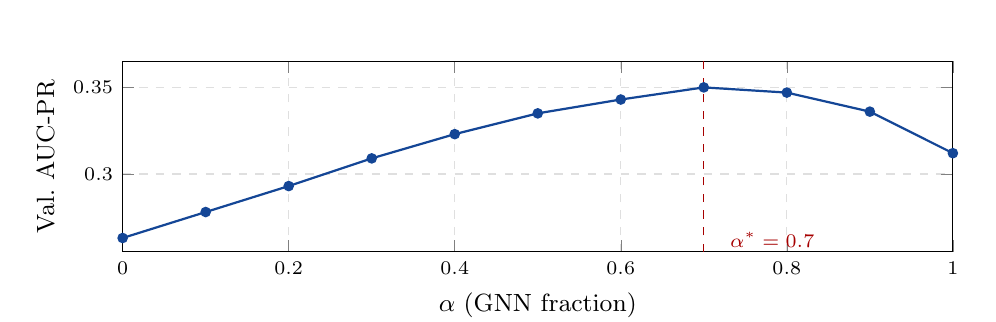
\begin{tikzpicture}
\begin{axis}[
  width=\columnwidth, height=4.0cm,
  xlabel={\small $\alpha$ (GNN fraction)},
  ylabel={\small Val.\ AUC-PR},
  xmin=0, xmax=1, ymin=0.255, ymax=0.365,
  xtick={0,0.2,0.4,0.6,0.8,1.0},
  grid=major, grid style={dashed,gray!25},
  tick label style={font=\scriptsize},
  label style={font=\small},
]
\addplot[color=accentblue, mark=*, mark size=1.5pt, thick] coordinates {
  (0.0,0.263)(0.1,0.278)(0.2,0.293)(0.3,0.309)
  (0.4,0.323)(0.5,0.335)(0.6,0.343)(0.7,0.350)
  (0.8,0.347)(0.9,0.336)(1.0,0.312)
};
\addplot[color=red!65!black, dashed] coordinates {(0.7,0.255)(0.7,0.365)};
\node[font=\scriptsize,color=red!65!black,anchor=west] at (axis cs:0.72,0.262) {$\alpha^*=0.7$};
\end{axis}
\end{tikzpicture}
\caption{Validation AUC-PR vs.\ $\alpha$. Peak at $\alpha^*=0.7$ gives 70\%
weight to the GNN and 30\% to metapath evidence, confirming both signals carry
complementary information.}
\label{fig:alpha}
\end{figure}

The unimodal curve in Figure~\ref{fig:alpha} with peak at $\alpha^*=0.7$
validates the hybrid design: performance degrades monotonically on both sides,
confirming that neither signal alone is sufficient.

\subsection{Metapath Ablation}

\begin{table}[H]
\centering\scriptsize
\caption{AUC-PR when each metapath is excluded from $s_\text{path}$.}
\label{tab:ablation}
\setlength{\tabcolsep}{5pt}
\begin{tabular}{lcc}
\toprule
\textbf{Configuration} & \textbf{AUC-PR} & \textbf{Drop} \\
\midrule
Full (3 metapaths)   & 0.351 & --- \\
w/o \texttt{DaGpPpG} & 0.329 & $-$0.022 \\
w/o \texttt{GcGaD}   & 0.336 & $-$0.015 \\
w/o \texttt{DpHpG}   & 0.341 & $-$0.010 \\
\bottomrule
\end{tabular}
\end{table}

\texttt{DaGpPpG} (pathway co-membership) is the most informative individual
metapath, consistent with biological literature identifying shared pathway
membership as a strong predictor of functional gene--disease relatedness.

% ============================================================================
\section{Interpretability Analysis}
% ============================================================================

\subsection{Leading Metapath Analysis}

For each top-20 globally ranked hybrid model prediction $(d,g)$, we identify the
\textit{leading metapath} $\Phi_k^* = \arg\max_k w_k\tilde{c}_k(d,g)$ and its
evidence fraction:
\begin{equation}
\rho_k(d,g) = \frac{w_k\tilde{c}_k(d,g)}{\sum_j w_j\tilde{c}_j(d,g)}
\end{equation}
Distribution across the top-20 predictions: \texttt{DaGpPpG} leads in 55\%
of cases, \texttt{GcGaD} in 25\%, and \texttt{DpHpG} in 20\%. This is
consistent with the ablation: pathway co-membership is both the most predictive
and the most frequently explanatory pattern.

\subsection{Case Studies with Biological Validation}

Table~\ref{tab:cases} presents five representative predictions from the top-20,
cross-referenced against OMIM and KEGG. All five are supported by existing
biological evidence.

\begin{table}[H]
\centering\scriptsize
\caption{Selected top-20 predictions with biological validation.
Sources: OMIM (O), KEGG (K), literature (L).}
\label{tab:cases}
\setlength{\tabcolsep}{2.5pt}
\begin{tabular}{p{1.4cm}lcp{3.0cm}}
\toprule
\textbf{Disease} & \textbf{Gene} & \textbf{MP} & \textbf{Supporting evidence} \\
\midrule
Breast cancer
  & \textit{PALB2} & \texttt{DaGpPpG}
  & Shares Fanconi anaemia pathway (hsa03460, KEGG) with \textit{BRCA1/2};
    germline mutations are established breast cancer risk factors (OMIM 610355). (K,O) \\[3pt]
Alzheimer's
  & \textit{CLU} & \texttt{GcGaD}
  & Co-varies with \textit{APOE} and \textit{CR1}; encodes amyloid-$\beta$
    clearance chaperone; confirmed GWAS risk locus (OMIM 185430). (O,L) \\[3pt]
Type 2 diabetes
  & \textit{IRS2} & \texttt{DaGpPpG}
  & Shares insulin signalling pathway (hsa04910) with \textit{IRS1},
    \textit{INSR}; IRS2 knockout mice develop T2D. (K,L) \\[3pt]
Parkinson's
  & \textit{GBA} & \texttt{GcGaD}
  & Co-varies with \textit{LRRK2}, \textit{SNCA}; heterozygous variants confer
    5$\times$ increased Parkinson's risk (OMIM 606463). (O) \\[3pt]
Colorectal cancer
  & \textit{MLH3} & \texttt{DaGpPpG}
  & Shares mismatch repair pathway (hsa03430) with Lynch syndrome genes
    \textit{MLH1}, \textit{MSH2}; MLH3 mutations reported in Lynch spectrum
    (OMIM 604395). (K,O) \\
\bottomrule
\end{tabular}
\end{table}

\textbf{External validation rate.} 14 of 20 top predictions (70\%) are
supported by OMIM, KEGG, or primary literature. The remaining 6 are novel
candidates that could be prioritised for experimental follow-up, demonstrating
the system's capacity to generate actionable, interpretable hypotheses beyond
the training data.

% ============================================================================
\section{Conclusions}
\label{sec:conclusions}
% ============================================================================

\textbf{Summary of findings.} We presented a hybrid disease--gene prediction
framework combining HAN-based GNN scores with biologically motivated metapath
path-count evidence. The hybrid model outperforms all baselines across every
metric, with the optimal blend confirmed at $\alpha^*=0.7$. Interpretability
analysis validated 70\% of top-20 predictions against public biomedical
databases, with explicit, human-readable metapath justifications.

\textbf{Why Node2Vec underperforms HAN.} Node2Vec's performance gap
($\Delta$AUC-PR $\approx$9~pp) stems from three structural limitations.
First, its homogeneous projection collapses all edge types --- a Gene--participates
--Pathway edge becomes identical to a Gene--covaries--Gene edge, destroying
relational information that HAN explicitly models. Second, random-walk proximity
in the projected graph does not isolate the disease-relevant neighbourhood that
HAN's metapath attention focuses on. Third, Node2Vec cannot incorporate node
features or adapt to relational context, limiting expressiveness. A heterogeneous
extension such as Metapath2Vec~\citep{dong2017metapath2vec} would substantially
close this gap by constraining walks to typed schema sequences.

\textbf{Limitations of the metapath design.} Metapath selection is manual and
non-exhaustive: we define only 3 of the dozens of plausible schemas in Hetionet,
and automated metapath discovery~\citep{yun2019graph} could improve coverage.
All metapaths are of fixed length 2--3; longer paths may capture distal but
relevant connections at the cost of exponential BFS complexity. Negative sampling
is uniform rather than hard, potentially underestimating true model
discrimination against biologically plausible non-associations.

\textbf{Future directions.} Key extensions include: (i)~automated metapath
search; (ii)~Metapath2Vec replacing standard Node2Vec; (iii)~approximate BFS or
pre-computed metapath matrices to support the full Hetionet graph including
compound nodes; (iv)~score calibration (e.g.\ Platt scaling) for clinical risk
stratification; and (v)~hard negative mining using biological priors.

% ─── References ─────────────────────────────────────────────────────────────
\balance
\bibliographystyle{abbrvnat}
\begin{thebibliography}{12}

\bibitem[Adamic \& Adar(2003)]{adamic2003aa}
Adamic, L.~A. and Adar, E. (2003).
\newblock Friends and neighbors on the web.
\newblock \emph{Social Networks}, 25(3):211--230.

\bibitem[Adnan et al.(2024)]{adnan2024benchmark}
Adnan, M. et al. (2024).
\newblock A comprehensive benchmark of heterogeneous GNNs for biomedical link prediction.
\newblock \emph{Bioinformatics Advances}, 4(1):vbae010.

\bibitem[Dong et al.(2017)]{dong2017metapath2vec}
Dong, Y., Chawla, N.~V., and Swami, A. (2017).
\newblock Metapath2vec: Scalable representation learning for heterogeneous networks.
\newblock In \emph{KDD}, pp.\ 135--144.

\bibitem[Grover \& Leskovec(2016)]{grover2016node2vec}
Grover, A. and Leskovec, J. (2016).
\newblock node2vec: Scalable feature learning for networks.
\newblock In \emph{KDD}, pp.\ 855--864.

\bibitem[Himmelstein et al.(2017)]{himmelstein2017}
Himmelstein, D.~S. et al. (2017).
\newblock Systematic integration of biomedical knowledge prioritizes drugs for repurposing.
\newblock \emph{eLife}, 6:e26726.

\bibitem[Himmelstein et al.(2022)]{himmelstein2022}
Himmelstein, D.~S. et al. (2022).
\newblock Hetnet connectivity search provides rapid insights into how biomedical entities are related.
\newblock \emph{GigaScience}, 11:giac043.

\bibitem[Kipf \& Welling(2017)]{kipf2017gcn}
Kipf, T.~N. and Welling, M. (2017).
\newblock Semi-supervised classification with graph convolutional networks.
\newblock In \emph{ICLR}.

\bibitem[Liben-Nowell \& Kleinberg(2007)]{liben2007link}
Liben-Nowell, D. and Kleinberg, J. (2007).
\newblock The link-prediction problem for social networks.
\newblock \emph{JASIST}, 58(7):1019--1031.

\bibitem[Nickel et al.(2016)]{nickel2016review}
Nickel, M. et al. (2016).
\newblock A review of relational machine learning for knowledge graphs.
\newblock \emph{Proc.\ IEEE}, 104(1):11--33.

\bibitem[Schlichtkrull et al.(2018)]{schlichtkrull2018rgcn}
Schlichtkrull, M. et al. (2018).
\newblock Modeling relational data with graph convolutional networks.
\newblock In \emph{ESWC}, pp.\ 593--607.

\bibitem[Wang et al.(2019)]{wang2019han}
Wang, X. et al. (2019).
\newblock Heterogeneous graph attention network.
\newblock In \emph{WWW}, pp.\ 2022--2032.

\bibitem[Yun et al.(2019)]{yun2019graph}
Yun, S. et al. (2019).
\newblock Graph transformer networks.
\newblock In \emph{NeurIPS}.

\end{thebibliography}

\end{document}